\section{Result and Analyze}
We first test our feature extraction and tracking algorithm on a 256*256*256 vortex data set obtained from a combustion solver that can simulate turbulent flames. In this data set, each voxel represents the magnitude of vorticity derived from velocity using a curl operator. As time evolves, vortical features may vary from small amassed blob features to long curly features that span over large portion of the volume, as depicted in Figure~\ref{fig:combustion-labeled}.

\begin{figure}[!htp]
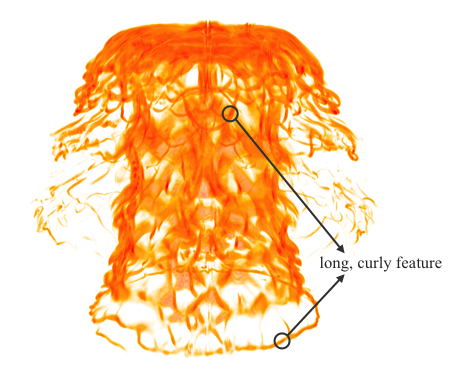
\includegraphics[width=0.9\linewidth]{combustion_labeled.png}
\caption{The rendering result of a single time step }
\label{fig:combustion-labeled}
\end{figure}

\subsection{Performance Result}
The volume data could be generated either in advance or on the fly, hence here we ignore the I/O cost and only focus on the computation time of the following three portions.

1. Extracting Features ($T_{extract}$);

Since we use the region-growing based algorithm to extract features, the computation time is mainly determined by the scale of the volume as well as the number of processors being used. Once the raw volume data and how it is partitioned, a.k.a. the size of each data block is determined, the computation time for extracting residing features remains approximately the same. For pre-generated data set, the size of each data block decreases as the number of processors increases and hence so does the time spent on extracting features. As depicted in Figure~\ref{fig:feature-extraction} $T_{extract}$ is approximately log-linear decreased as the number of processors grows from 8 to 16384;

\begin{figure}[ht]
	\centering
	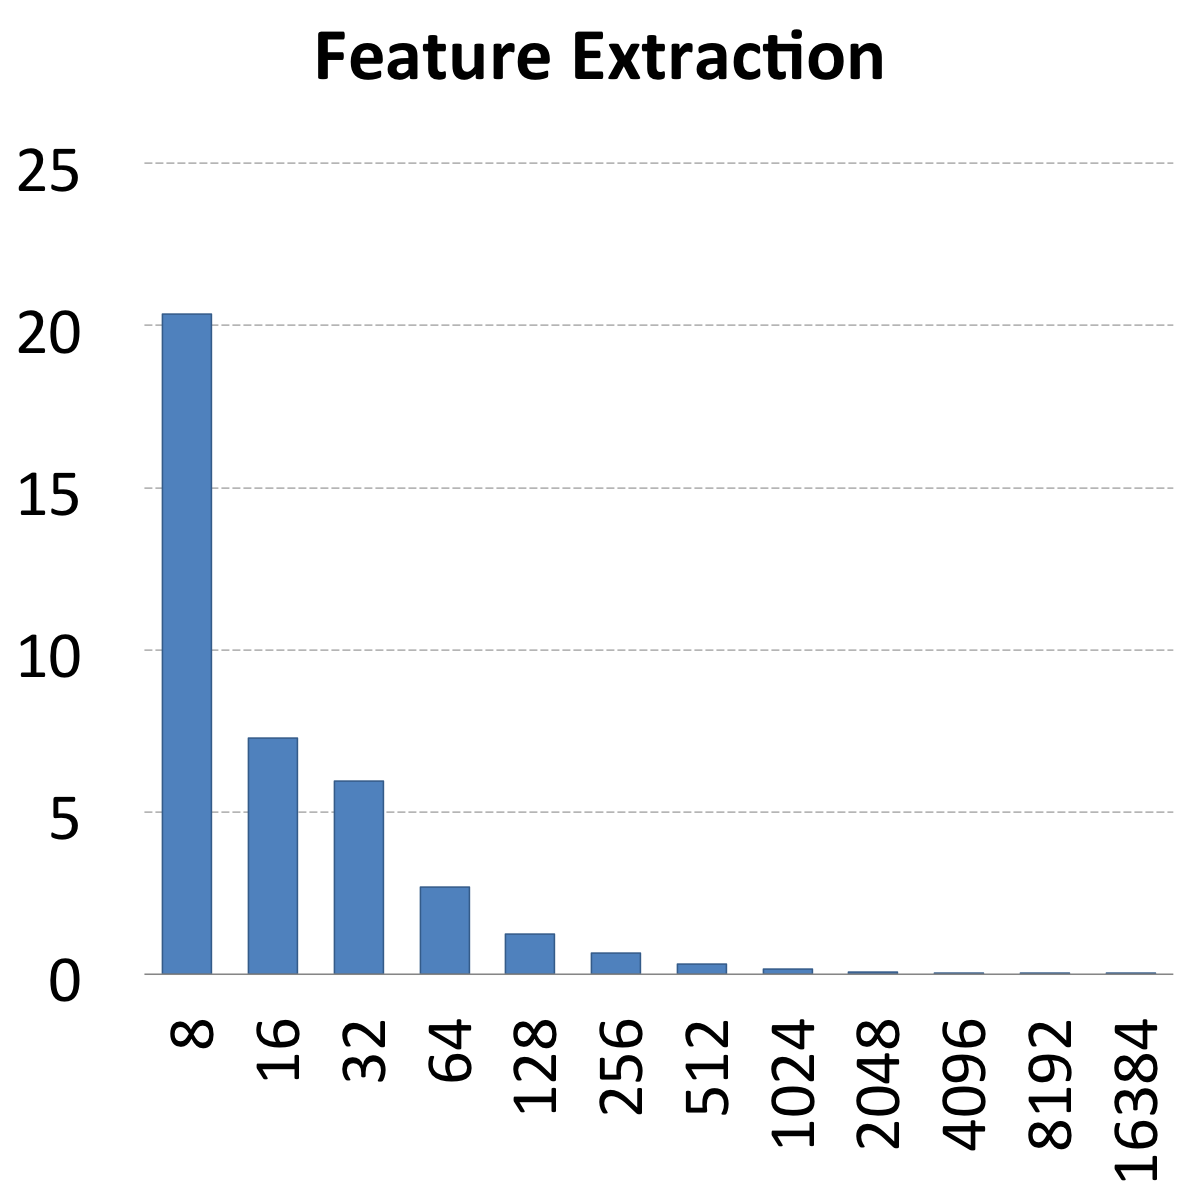
\includegraphics[width=0.45\linewidth]{feature_extraction.png}
	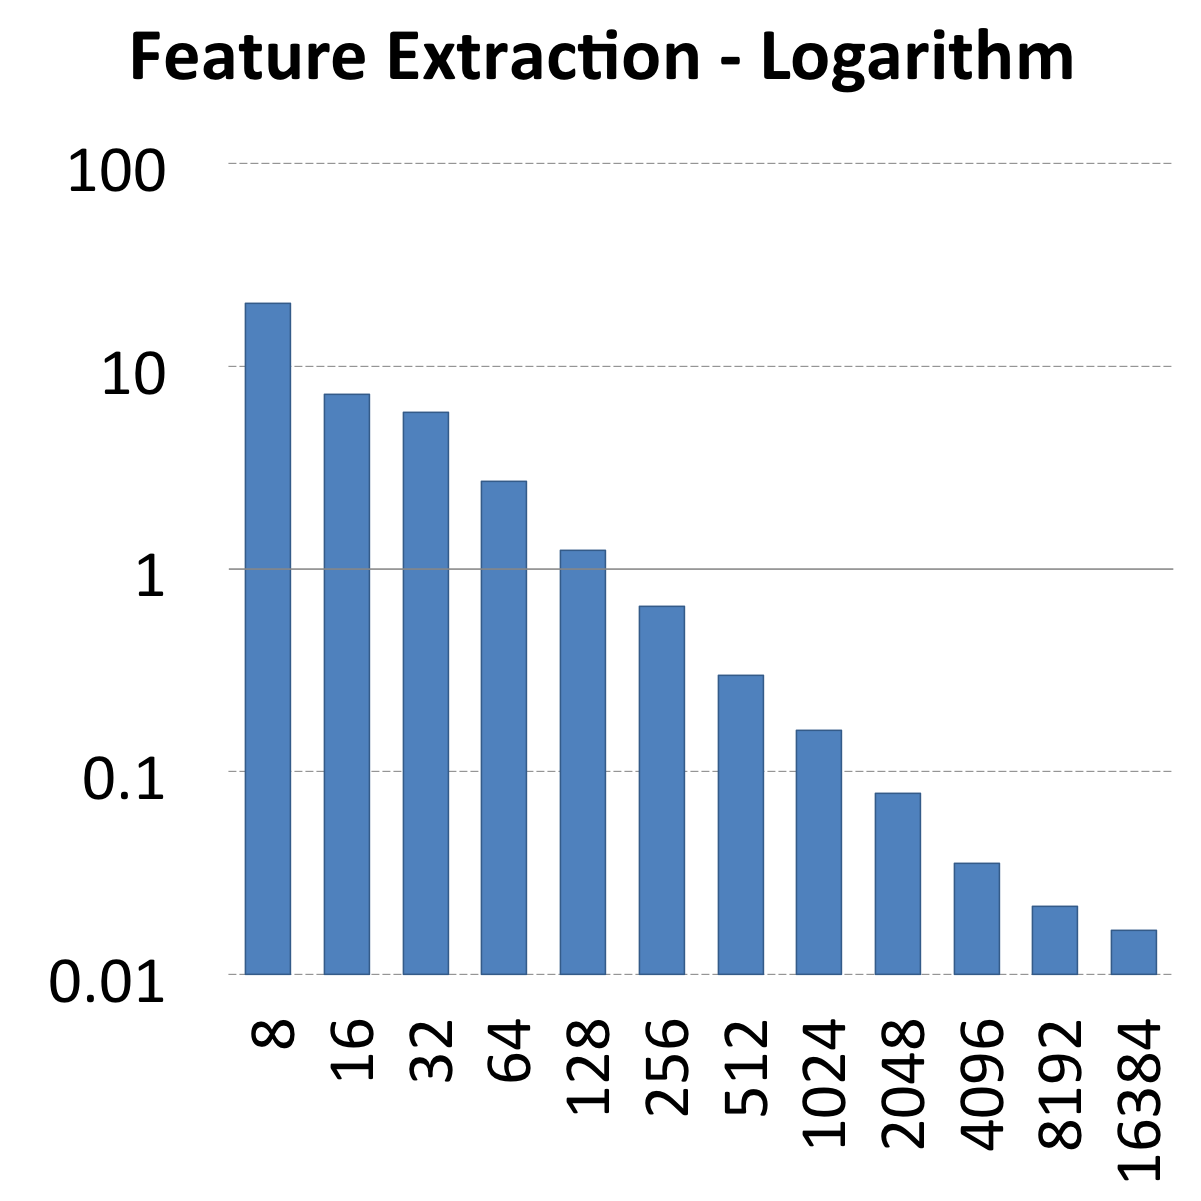
\includegraphics[width=0.45\linewidth]{feature_extraction_log.png}
	\caption{Computation time for feature extraction, log-linearly scalable as the number of processor increases}
	\label{fig:feature-extraction}
\end{figure}

2. Create Local Connectivity Graph ($T_{create}$);

Despite the size of each data block, the computational cost for creating and updating local connectivity graph is dependent on the number of the features extracted within the original volume, or more precisely, the number of features that touches the boundary surface of their residing data block. Similar to $T_{extract}$, $T_{create}$ will decrease as the number of processors increases for pre-generated data set, as the the number of feature-on-boundary decreases accordingly. For the combustion data set, it takes an average of 0.1 seconds to create the local connectivity graph, approximately 0.5\% the time of $T_{extract}$ using the same amount of processors. This portion increases but does not succeed 1\% in out test, hence $T_{create}$ is not considered a bottleneck for the pre-generated data set. \textcolor{red}{for in-situ visualization however... }

\begin{figure}[ht]
	\centering
	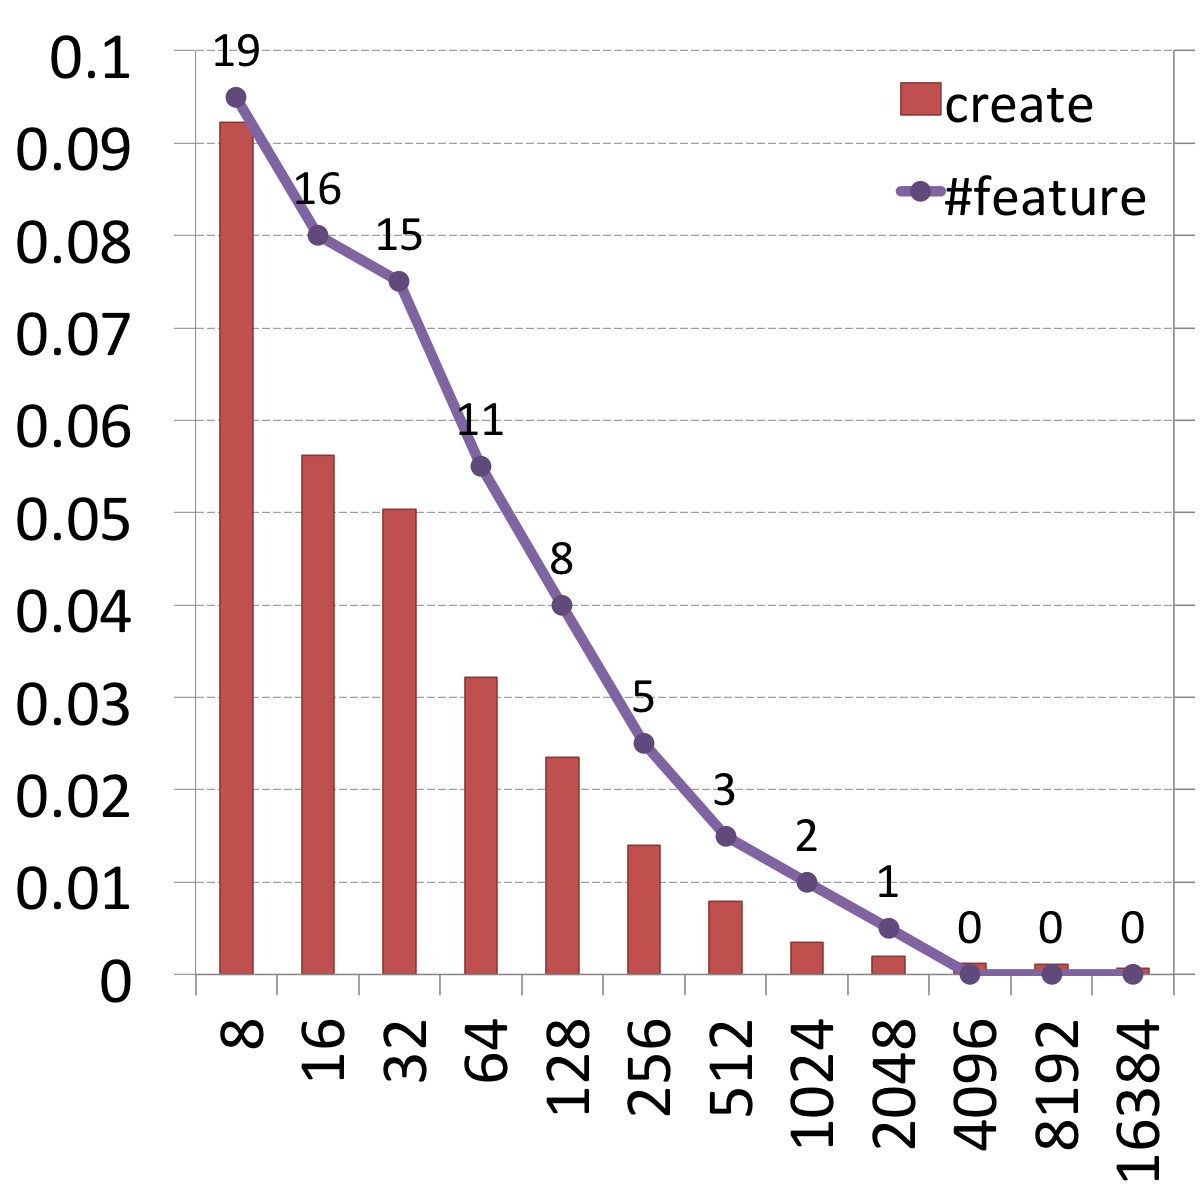
\includegraphics[width=0.45\linewidth]{create_local_graph.png}
	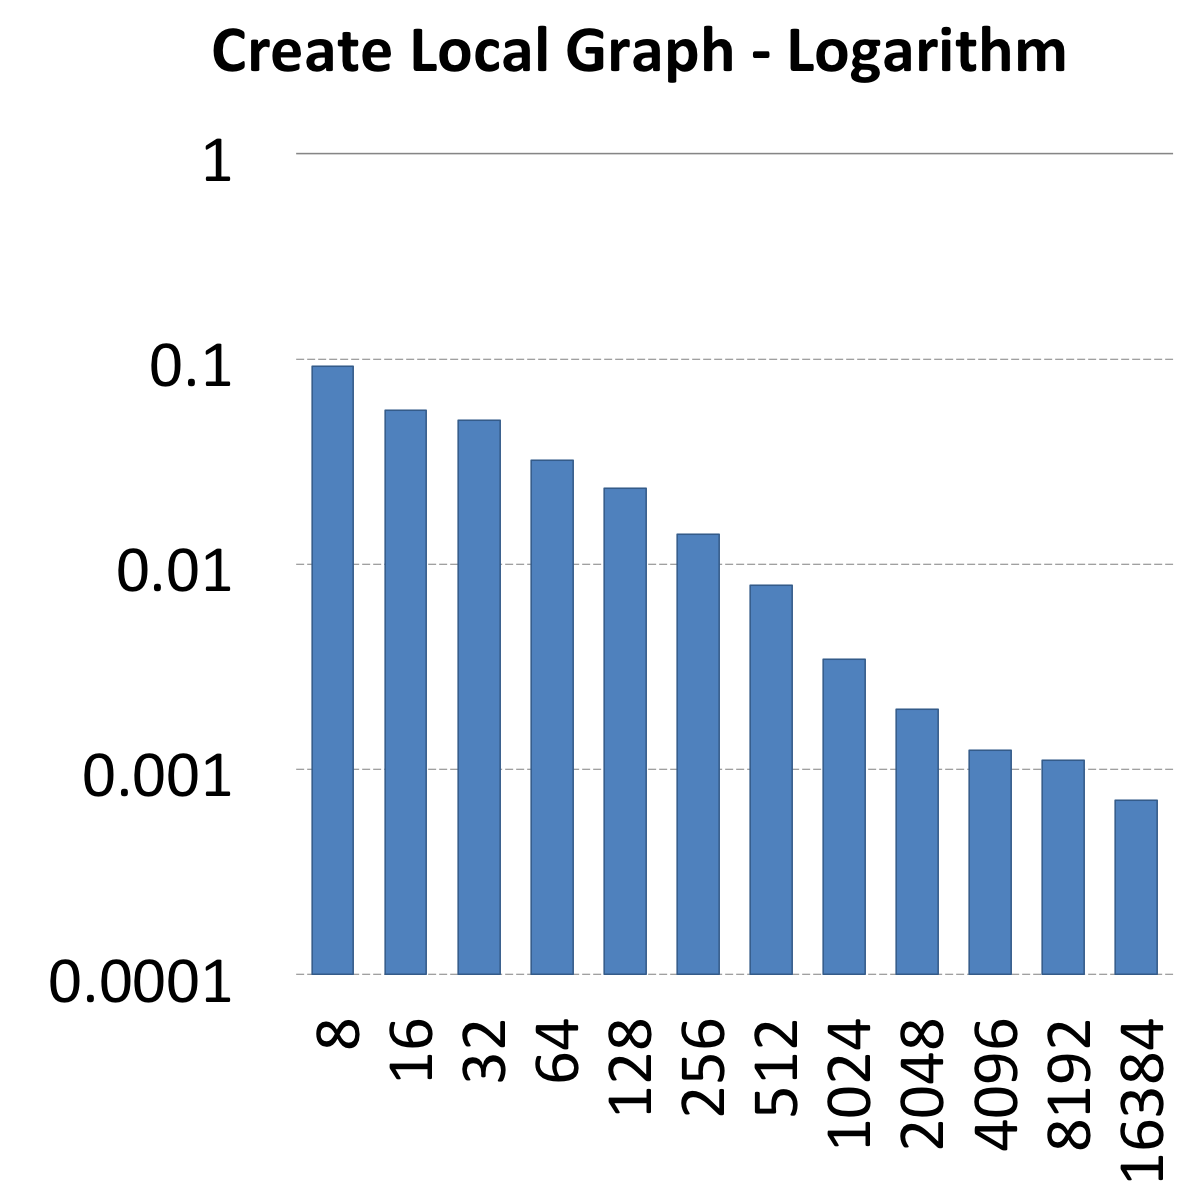
\includegraphics[width=0.45\linewidth]{create_local_graph_log.png}
	\caption{Computation time for creating local connectivity tree, log-linearly scalable as the number of processor increases and the time is approximately proportional to the number of features-on-boundary}
	\label{fig:create-local-graph}
\end{figure}

3. Merge Local Connectivity Graph ($T_{merge}$)

The three \textcolor{red}{(only the first two are tested for now)} merging strategies are the major factors of the scalability of our algorithm. Though the number of feature-on-boundary decreases as more processors involved, the communication time for the Global-Merge approach increases as $N_p$ increases. The total temporal cost $T_{global}$ for Global-Merge exceeds $T_{extract}$ after certain amount of processors, 2048 for the combustion data set, which makes the overall computation time rebounds (Figure~\ref{fig:global-merge}). The Local-Merge approach on the other hand, scaled well up to 16384 processors for the combustion data set, as the communicational cost is as low as ${O(\sqrt[3]{N_p})}$. (Figure~\ref{fig:local-merge}).

Also from the comparison of the computational cost as depicted in Figure~\ref{fig:local-vs-global}, we can see that the Global-Merge is suitable for scenarios that we only need a small cluster of processors, and Local-Merge for creating connectivity graph using a relatively large amount of the processors.

\begin{figure}[ht]
	\centering
	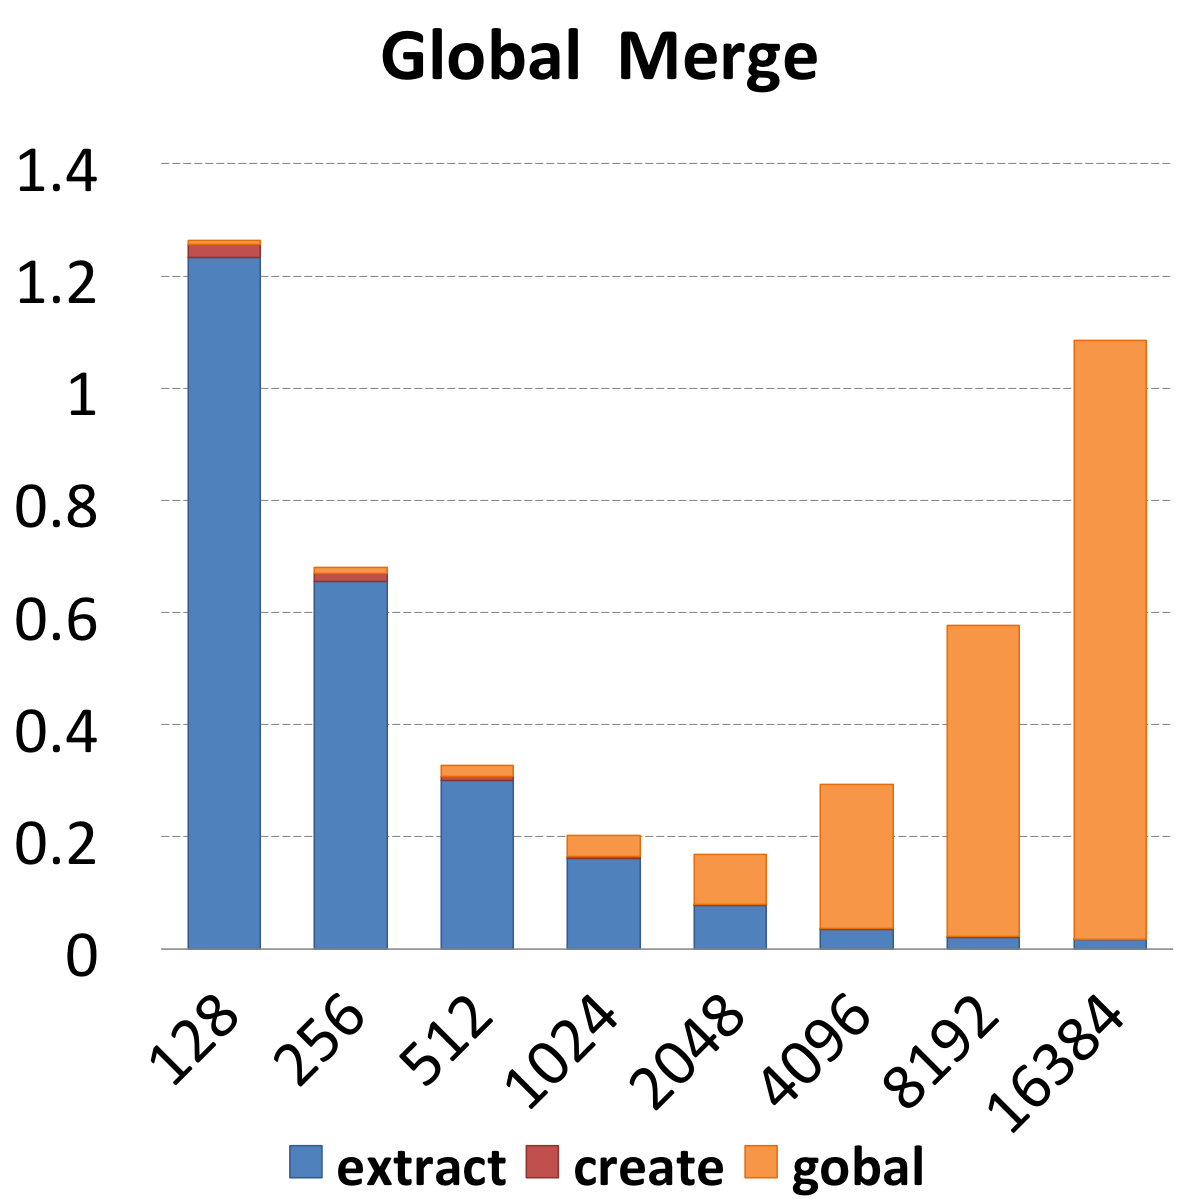
\includegraphics[width=0.45\linewidth]{global_merge.png}
	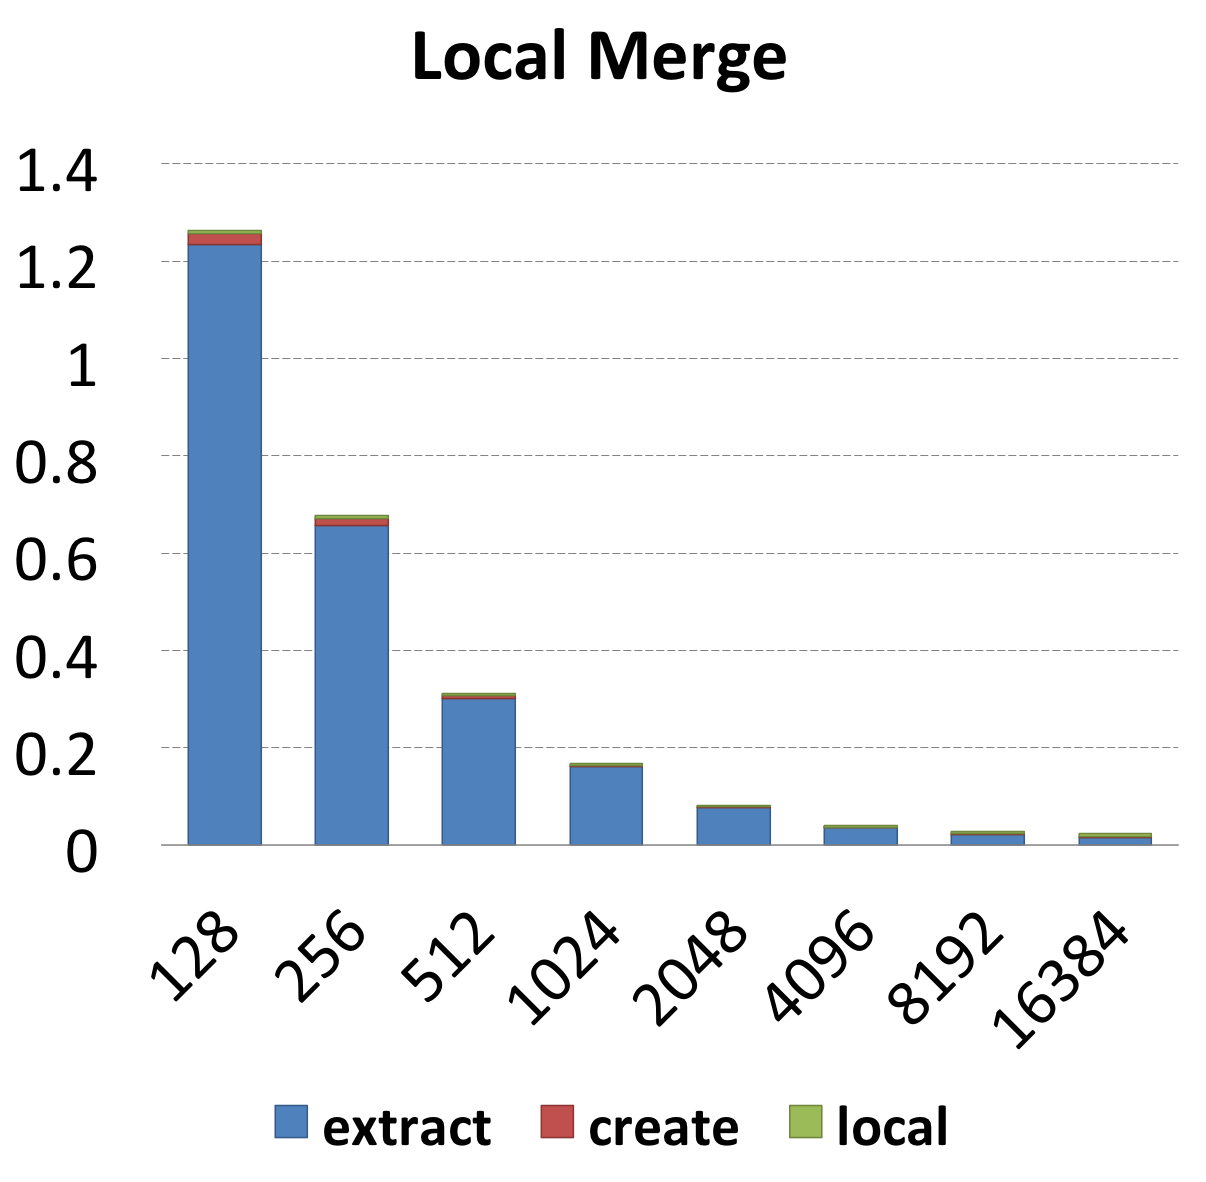
\includegraphics[width=0.45\linewidth]{local_merge.png}
	\caption{Total computation time comparison for different merging strategy. The decentralized-global-merge strategy scaled up to 2048 processors but the merging time outweighs the extraction time when using more processors; The decentralized-local-merge strategy scaled log-linearly up 16384 processors for the combustion data set.}
	\label{fig:global-merge}
\end{figure}

\begin{figure}[ht]
	\centering
	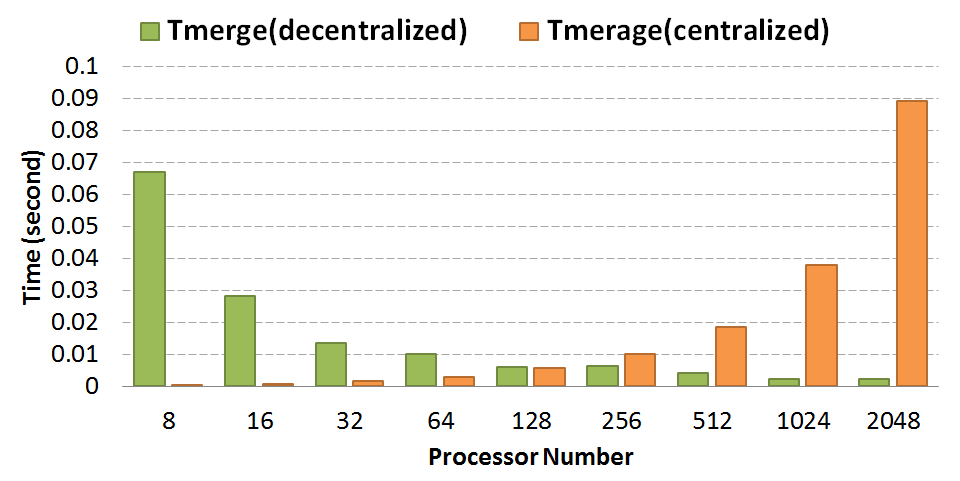
\includegraphics[width=0.45\linewidth]{local_vs_global.png}
	\caption{The comparison between the computation time for the local and global merging strategy. The global merge strategy works well for a small number of processors while the local merge exceeds after a certain number, as for the combustion data set, 128 processors, is used.}
	\label{fig:local-vs-global}
\end{figure}
